% !TEX program = lualatex
\documentclass[border=6pt]{standalone}
% ---------------------------------------------------------------------------
% tikzpreamble.tex -- shared by main.tex and by every standalone in tikz/
% ---------------------------------------------------------------------------
\usepackage{amsmath}
\usepackage{amssymb}
\usepackage{tikz}
\usepackage{circuitikz}
\usetikzlibrary{arrows.meta,calc,positioning,decorations.pathmorphing,decorations.pathreplacing,
                decorations.markings,patterns,angles,quotes,fit,
                shapes.geometric,shapes.misc,backgrounds,intersections}

\ctikzset{bipoles/length=0.85cm}
\ctikzset{resistors/scale=0.85}
\ctikzset{capacitors/scale=0.9}

\tikzset{
  wire/.style      = {line width=0.7pt},
  dashedwire/.style= {line width=0.7pt, densely dashed},
  term/.style      = {circle, draw, line width=0.6pt, fill=white,
                      inner sep=0pt, minimum size=4.5pt},
  node dot/.style  = {circle, fill=black, inner sep=0pt, minimum size=4pt},
  boxlabel/.style  = {font=\sffamily\small},
  annot/.style     = {font=\small, align=left},
  phasor/.style    = {-{Stealth[length=3.2mm,width=2.2mm]}, line width=1.1pt},
  thinphasor/.style= {-{Stealth[length=2.6mm,width=1.8mm]}, line width=0.7pt},
  axis line/.style = {-{Stealth[length=2.6mm,width=1.8mm]}, line width=0.6pt},
  guide/.style     = {densely dashed, line width=0.4pt, gray},
}
\usepackage{siunitx}

\begin{document}
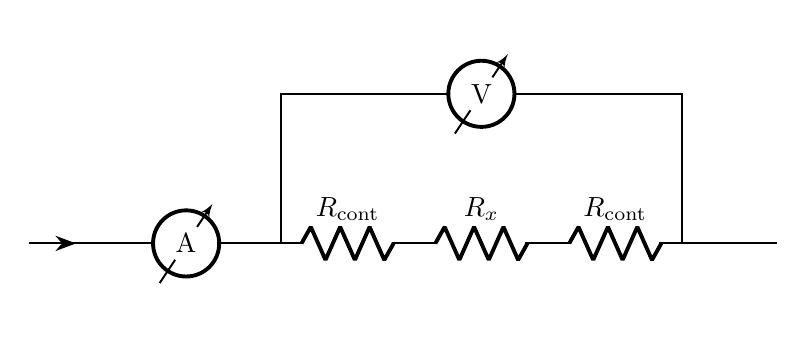
\begin{tikzpicture}
  \draw[wire] (-1.2,0) -- (0,0);
  \draw[-{Stealth[length=2.6mm]},line width=0.7pt] (-1.2,0) -- (-0.6,0);
  \draw[wire] (0,0) to[rmeterwa, t=A] (1.6,0) -- (2.0,0)
              to[R=$R_{\mathrm{cont}}$] (3.7,0)
              to[R=$R_x$] (5.4,0)
              to[R=$R_{\mathrm{cont}}$] (7.1,0) -- (8.3,0);
  \draw[wire] (2.0,0) -- (2.0,1.9) to[rmeterwa, t=V] (7.1,1.9) -- (7.1,0);
\end{tikzpicture}
\end{document}
